\documentclass[12pt,fullpage,letterpaper]{article}

\newenvironment{proof}{\noindent{\bf Proof:}}{\qed\bigskip}

\newtheorem{theorem}{Theorem}
\newtheorem{corollary}{Corollary}
\newtheorem{lemma}{Lemma} 
\newtheorem{claim}{Claim}
\newtheorem{fact}{Fact}
\newtheorem{definition}{Definition}
\newtheorem{assumption}{Assumption}
\newtheorem{observation}{Observation}
\newtheorem{example}{Example}
\newcommand{\qed}{\rule{7pt}{7pt}}

\newcommand{\assignment}[4]{
\thispagestyle{plain} 
\newpage
\setcounter{page}{1}
\noindent
\begin{center}
\framebox{ \vbox{ \hbox to 6.28in
{\bf CS446: Machine Learning \hfill #1}
\vspace{4mm}
\hbox to 6.28in
{\hspace{2.5in}\large\mbox{Problem Set #2}}
\vspace{4mm}
\hbox to 6.28in
{{\it Handed Out: #3 \hfill Due: #4}}
}}
\end{center}
}


\newcommand{\handout}[3]{
\thispagestyle{plain} 
\newpage
\setcounter{page}{1}
\noindent
\begin{center}
\framebox{ \vbox{ \hbox to 6.28in
{\bf CS446: Machine Learning \hfill #1}
\vspace{4mm}
\hbox to 6.28in
{\hspace{2.5in}\large\mbox{#2}}
\vspace{4mm}
\hbox to 6.28in
{{\it Handed Out: #3 \hfill Name (NetID): \rule[-2pt]{4cm}{0.1pt} }}
}}
\end{center}
}


\newcommand{\assgsoln}[4]{
\thispagestyle{plain} 
\newpage
\setcounter{page}{1}
\noindent
\begin{center}
\framebox{ \vbox{ \hbox to 6.28in
{\bf CS446: Machine Learning \hfill #1}
\vspace{4mm}
\hbox to 6.28in
{\hspace{2.5in}\large\mbox{Problem Set #2 Solutions}}
\vspace{4mm}
\hbox to 6.28in
{{\it Handed Out: #3 \hfill Handed In: #4}}
}}
\end{center}
}


\newcommand{\solution}[4]{
\thispagestyle{plain} 
\newpage
\setcounter{page}{1}
\noindent
\begin{center}
\framebox{ \vbox{ \hbox to 6.28in
{\bf CS446: Machine Learning \hfill #4}
\vspace{4mm}
\hbox to 6.28in
{\hspace{2.5in}\large\mbox{Problem Set #3}}
\vspace{4mm}
\hbox to 6.28in
{#1 \hfill {\it Handed In: #2}}
}}
\end{center}
\markright{#1}
}


\newenvironment{algorithm}
{\begin{center}
\begin{tabular}{|l|}
\hline
\begin{minipage}{1in}
\begin{tabbing}
\quad\=\qquad\=\qquad\=\qquad\=\qquad\=\qquad\=\qquad\=\kill}
{\end{tabbing}
\end{minipage} \\
\hline
\end{tabular}
\end{center}}

\def\Comment#1{\textsf{\textsl{$\langle\!\langle$#1\/$\rangle\!\rangle$}}}


\usepackage{amsmath}
\usepackage{algorithm}% http://ctan.org/pkg/algorithm
\usepackage{algpseudocode}% http://ctan.org/pkg/algorithmicx
\usepackage{graphicx}
\usepackage{listings}
\graphicspath{ {.} }

\DeclareMathOperator{\proj}{proj}
\newcommand{\vctproj}[2][]{\proj_{\vec{#1}}\vec{#2}}

\sloppy
\newcommand{\ignore}[1]{}
\newcommand{\bx}{{\bf x}}
\newcommand{\bw}{{\bf w}}

\newcommand{\bb}[1]{{\bf #1}}
\newcommand{\pp}{\noindent}
\newcommand{\ov}{\overline}
\renewcommand{\labelitemii}{\tiny$\circ$}

\oddsidemargin 0in
\evensidemargin 0in
\textwidth 6.5in
\topmargin -0.5in
\textheight 9.0in

\begin{document}

\solution{Bangqi Wang}{\today}{5}{Spring 2017}
% Fill in the above, for example, as follows:
% \solution{Joe Smith}{\today}{1}{Fall 2012}

\pagestyle{myheadings}  % Leave this command alone

\begin{enumerate}
\item[1.] Answer to problem 1
	\begin{enumerate}
	\item[a.]
		For this question, I will use $i$, $j$, $k$ to represent input, hidden, and output layers:
		\begin{eqnarray}
		\frac{\partial E_d}{\partial w_{jk}} = && \frac{\partial E_d}{\partial o_k} \frac{\partial o_k}{\partial h_k} \frac{\partial h_k}{\partial w_{jk}}\\
		\frac{\partial E_d}{\partial o_k} = && -(t_k - o_k)\\
		\frac{o_k}{h_k} = && 
			\begin{cases}
			0, \: h_k \leq 0\\
			1, \: h_k > 0
			\end{cases}\\
		\frac{h_k}{w_{kl}} = && x_j\\
		\Rightarrow w_{jk} \leftarrow && w_{jk} + \gamma \sigma_k x_j\\
		where, && \: \sigma_k = \frac{\partial E_d}{\partial h_k} = 
			\begin{cases}
			0, \: h_k\leq0\\
			-(t_k-o_k), \: h_k>0
			\end{cases}\\
		&& \gamma \text{ is the learning rate}
		\end{eqnarray}

		\begin{eqnarray}
		\frac{\partial E_d}{\partial w_{ij}} = && \frac{\partial E_d}{\partial h_j} \frac{\partial h_j}{\partial w_{ij}}\\
		= &&\sum_{k \in downstream(j)} \frac{\partial E_d}{\partial h_k} \frac{\partial h_k}{\partial h_j} \frac{\partial h_j}{\partial w_{ij}}\\
		\frac{\partial E_d}{\partial h_k} = && -\sigma_k\\
		\frac{\partial h_k}{\partial h_j} = && 
			\begin{cases}
			0, \: h_j \leq0\\
			w_{jk}, \: h_j > 0
			\end{cases}\\
		\frac{\partial h_j}{\partial w_{ij}} = && x_i\\
		\Rightarrow w_{ij} \leftarrow && w_{ij} + \gamma \sigma_j x_i\\
		where, && \: \sigma_j = \frac{\partial E_d}{\partial w_{ij}} = 
			\begin{cases}
			0, \: h_j \leq 0\\
			\sum_{k \in downstream(j)} -\sigma_k w_{jk} x_i, \: h_j>0
			\end{cases}\\
		&& \gamma \text{ is the learning rate}
		\end{eqnarray}
	\pagebreak
	\item[b.]
		\begin{enumerate}
		\item[ii.] The tables below show the average accuracy for each parameter setting with ascending order for \textbf{CIRCLES} and \textbf{MNIST} datasets.
		\begin{enumerate}
		\item[\textbf{CIRCLES}] :
		\begin{center}
		\begin{tabular}{|l|l|l|l|l|}
		\hline
		Accuracy\% & batch\_size & activation     & learning\_rate       & layer\_width         \\ \hline\hline
		48.75    & 10          & relu           & 0.1                  & 50                   \\ \hline
		49       & 100         & tanh           & 0.01                 & 10                   \\ \hline
		49.75    & 50          & tanh           & 0.01                 & 10                   \\ \hline
		50.875   & 50          & tanh           & 0.01                 & 50                   \\ \hline
		52.125   & 100         & tanh           & 0.01                 & 50                   \\ \hline
		60.375   & 100         & relu           & 0.01                 & 10                   \\ \hline
		71.125   & 100         & tanh           & 0.1                  & 50                   \\ \hline
		72.5     & 10          & tanh           & 0.01                 & 50                   \\ \hline
		75.5     & 100         & tanh           & 0.1                  & 10                   \\ \hline
		78.375   & 10          & tanh           & 0.01                 & 10                   \\ \hline
		86.25    & 50          & tanh           & 0.1                  & 50                   \\ \hline
		91.25    & 50          & tanh           & 0.1                  & 10                   \\ \hline
		94.125   & 100         & relu           & 0.01                 & 50                   \\ \hline
		96.625   & 50          & relu           & 0.01                 & 10                   \\ \hline
		99.125   & 100         & relu           & 0.1                  & 10                   \\ \hline
		99.75    & 10          & relu           & 0.01                 & 10                   \\ \hline
		100      & 10          & relu           & 0.01                 & 50                   \\ \hline
		100      & 10          & relu           & 0.1                  & 10                   \\ \hline
		100      & 50          & relu           & 0.1                  & 10                   \\ \hline
		100      & 10          & tanh           & 0.1                  & 10                   \\ \hline
		100      & 10          & tanh           & 0.1                  & 50                   \\ \hline
		100      & 50          & relu           & 0.1                  & 50                   \\ \hline
		100      & 50          & relu           & 0.01                 & 50                   \\ \hline
		100      & 100         & relu           & 0.1                  & 50                   \\ \hline
		\end{tabular}
		\\Table: Average Accuracy for \textbf{CIRCLES}\\
		\end{center}
		.\\
		From the table above, we find that there are multiple parameter settings that can lead to $100\%$ accuracy. The best parameter settings are shown in the table below.
		\begin{center}
		\begin{tabular}{|l|l|l|l|l|}
		\hline
		Accuracy\% & batch\_size & activation     & learning\_rate       & layer\_width     \\ \hline\hline
		100      & 10          & relu           & 0.01                 & 50                   \\ \hline
		100      & 10          & relu           & 0.1                  & 10                   \\ \hline
		100      & 50          & relu           & 0.1                  & 10                   \\ \hline
		100      & 10          & tanh           & 0.1                  & 10                   \\ \hline
		100      & 10          & tanh           & 0.1                  & 50                   \\ \hline
		100      & 50          & relu           & 0.1                  & 50                   \\ \hline
		100      & 50          & relu           & 0.01                 & 50                   \\ \hline
		100      & 100         & relu           & 0.1                  & 50                   \\ \hline
		\end{tabular}
		\\Table: Best Parameter Settings for \textbf{CIRCLES}\\
		\end{center}
		\item[\textbf{MNIST}] :
		\begin{center}
		\begin{tabular}{|l|l|l|l|l|}
		\hline
		Accuracy\% & batch\_size & activation     & learning\_rate       & layer\_width         \\ \hline\hline
		51.16852385 & 10  & relu & 0.1  & 10 \\ \hline
		51.16852385 & 10  & relu & 0.1  & 50 \\ \hline
		95.70177429 & 50  & relu & 0.1  & 50 \\ \hline
		96.31951919 & 100 & tanh & 0.01 & 50 \\ \hline
		96.40294291 & 50  & tanh & 0.01 & 50 \\ \hline
		96.46133186 & 50  & relu & 0.1  & 10 \\ \hline
		96.54480431 & 10  & relu & 0.01 & 10 \\ \hline
		96.56152665 & 100 & tanh & 0.01 & 10 \\ \hline
		96.6032768  & 10  & tanh & 0.1  & 50 \\ \hline
		96.72844371 & 10  & tanh & 0.01 & 50 \\ \hline
		96.74506858 & 100 & relu & 0.1  & 50 \\ \hline
		96.76185358 & 50  & tanh & 0.01 & 10 \\ \hline
		96.84530514 & 50  & relu & 0.01 & 10 \\ \hline
		96.85365935 & 100 & relu & 0.1  & 10 \\ \hline
		96.86193002 & 10  & relu & 0.01 & 50 \\ \hline
		96.86197179 & 100 & tanh & 0.1  & 50 \\ \hline
		96.93709003 & 100 & relu & 0.01 & 50 \\ \hline
		96.95374972 & 50  & tanh & 0.1  & 50 \\ \hline
		96.96211089 & 50  & relu & 0.01 & 50 \\ \hline
		96.97885411 & 100 & relu & 0.01 & 10 \\ \hline
		97.1790975  & 100 & tanh & 0.1  & 10 \\ \hline
		97.1874517  & 10  & tanh & 0.01 & 10 \\ \hline
		97.24579192 & 10  & tanh & 0.1  & 10 \\ \hline
		97.30424352 & 50  & tanh & 0.1  & 10 \\ \hline
		\end{tabular}
		\\Table: Average Accuracy for \textbf{MNIST}\\
		\end{center}
		.\\
		From the table above, we find that there is a parameter setting that can lead to $97.3\%$ accuracy. The best parameter setting is shown below.
		\begin{center}
		\begin{tabular}{|l|l|l|l|l|}
		\hline
		Accuracy\% & batch\_size & activation     & learning\_rate       & layer\_width   \\ \hline\hline
		97.30424352 & 50  & tanh & 0.1  & 10 \\ \hline
		\end{tabular}
		\\Table: Best Parameter Setting for \textbf{MNIST}\\
		\end{center}
		\end{enumerate}
		\pagebreak
		\item[iii.] Learning curve:
			\begin{figure}[H]
				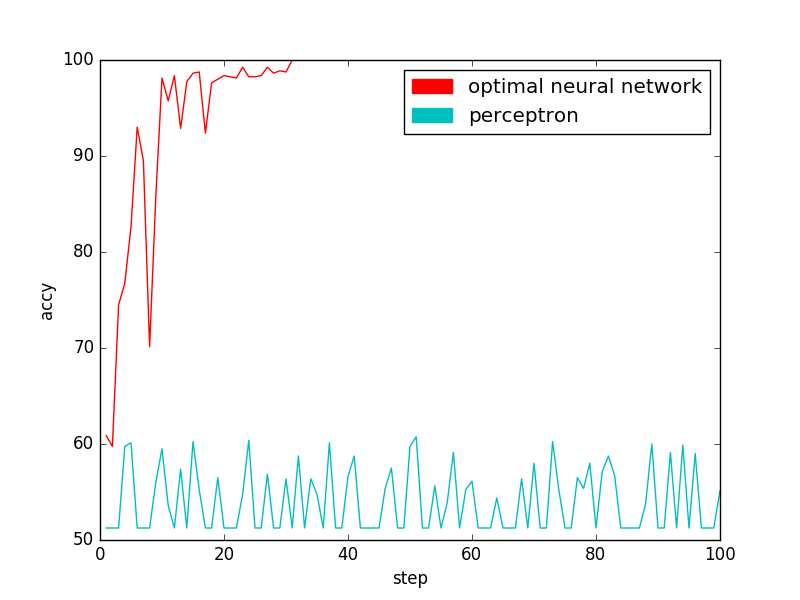
\includegraphics[width=\linewidth]{figure_circles.png}
				\caption{step vs accuracy for circle data}
			\end{figure}
			Accuracy of NN on the test data for CIRCLES: $100\%$\\
			Accuracy of Perceptron on the test data for CIRCLES: $49.7\%$\\\\
			For the dataset CIRCLES, NN has much better performance than Perceptron has. Since Perceptron is a linear seperator, it cannot seperate circle in two parts and the accuracy is around $50\%$ which is no better than random guess. For learning curve, NN has much smoother curve than Perceptron, and the curve keeps increasing gradually.
			\begin{figure}[H]
				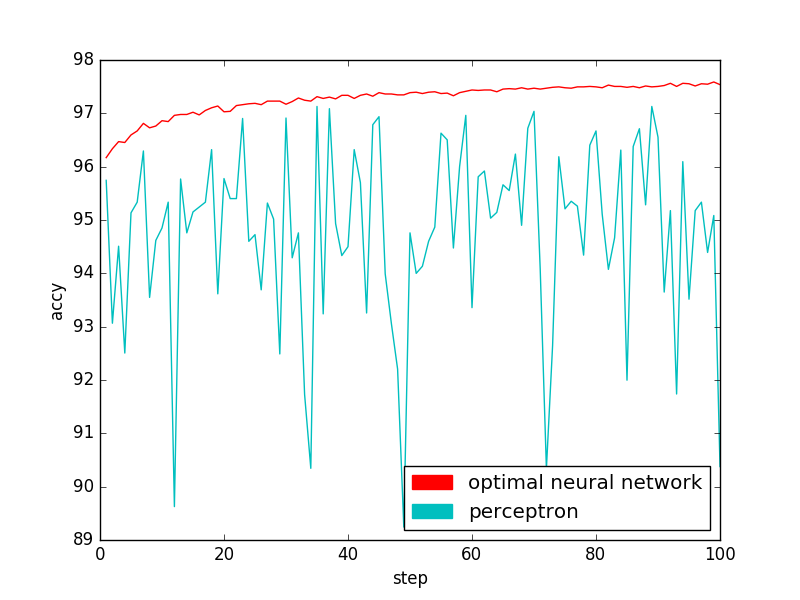
\includegraphics[width=\linewidth]{figure_mnist.png}
				\caption{step vs accuracy for circle data}
			\end{figure}
			Accuracy of NN on the test data for MNIST: $96.8\%$\\
			Accuracy of Perceptron on the test data for MNIST: $89.6\%$\\\\
			For the dataset MNIST, NN and Perceptron have similar performance. The performance of NN is slightly better than the performance of Perceptron. NN has numerous hidden layers and it could seperate the data more accurately. While, Perceptron is linear seperate that can only seperate the data in two parts with a line. Therefore, it is reasonable that NN has better performance than Perceptron. For the learning curve, NN has much smoother curve than Perceptron has. The learning curve of Perceptron vacilates dramatically.
		\end{enumerate}
	\end{enumerate}

\pagebreak
\item[2.] Answer to problem 2
	\begin{enumerate}
	\item[a.]
		\begin{enumerate}
		\item[i.] For \textbf{One-vs-All}: it learnt $k$ classifiers. \\
					For \textbf{All-vs-All}: it learnt $k^2$ classifiers.
		\item[ii.] For \textbf{One-vs-All}: it used $m$ samples. \\
					For \textbf{All-vs-All}: it used $\frac{2m}{k}$ samples.
		\item[iii.] For \textbf{One-vs-All}: it decided the label by the rule of winner takes all. \\
					For \textbf{All-vs-All}: it decided the label by the rule of majority vote.
		\item[iv.] For \textbf{One-vs-All}: it took $O(km)$ computational complexity.\\
					For \textbf{All-vs-All}: it took $O(k^2 \cdot \frac{2m}{k})$ = $O(km)$ computational complexity.
		\end{enumerate}
	\item[b.] I would prefer \textbf{One-vs-All}, because it is easier to implement, and has better performance efficiency-wise. \textbf{One-vs-All} evaluate $k$ linear classifiers and do Winner Takes All. While, \textbf{All-vs-All} evaluate $k^2$ linear classifiers. It has more expressivity, but less example to learnt from.
	\item[c.] Yes, using a KERNEL PERCEPTRON changes the analysis. The computational complexity increases by a factor of m. Therefore, \textbf{One-vs-All} is $O(km^2)$, and \textbf{All-vs-All} is $O(km^2)$. I would prefer to use \textbf{All-vs-All} when using a KERNEL PERCEPTRON, because it can learn from relatively small training set and work in the dual space more effectively.
	\item[d.] For \textbf{One-vs-All}: the overall training time complexities is $O(kdm^2)$. \\
			For \textbf{All-vs-All}: the overall training time complexities is $O(k^2d \cdot (\frac{2m}{k})^2)$ = $O(dm^2)$.\\
			In this situation, \textbf{All-vs-All} is the most efficient.
	\item[e.] For \textbf{One-vs-All}: the overall training time complexities is $O(kd^2m)$. \\
			For \textbf{All-vs-All}: the overall training time complexities is $O(k^2d^2 \cdot \frac{2m}{k})$ = $O(kd^2m)$.\\
			In this situation, \textbf{All-vs-All} and \textbf{One-vs-All} have same efficiency.
	\item[f.] For \textbf{Counting}: overall evaluation time complexities per example is $O(dm^2)$\\
			For \textbf{Knockout}: overall evaluation time complexities per example is $O(dm)$\\
	\end{enumerate}

\pagebreak
\item[3.] Answer to problem 3
	\begin{enumerate}
	\item[a.]
		\begin{enumerate}
		\item[i.] $E[A] = 1$\\
				$E[B] = \frac{1}{P_{boy}} = \frac{1}{0.5} = 2$ \\
		\item[ii.] The boy to girl ratio at the end of one generation in town is $1:1$.\\
		\end{enumerate}
	\item[b.]
		\begin{enumerate}
		\item[i.] 
			\[ P(A \cap B) = P(A|B) \cdot P(B) \]
			\[ P(A \cap B) = P(B|A) \cdot P(A) \]
			\[ P(A|B) \cdot P(B) = P(B|A) \cdot P(A) \]
			\[ P(A|B) = \frac{P(B|A) \cdot P(A)}{P(B)} \] \\
		\item[ii.]
			\begin{eqnarray}
			P(A \cap B \cap C) && = P(A \cap (B \cap C))\\
							   && = P(A|(B \cap C)) \cdot P(B \cap C)\\
							   && = P(A|(B \cap C)) \cdot (P(B|C) \cdot P(C))\\
							   && = P(A|B \cap C) \cdot P(B|C) \cdot P(C)
			\end{eqnarray}
		\end{enumerate}
	\item[c.] $E[X] = 1 \cdot P(A) + 0 \cdot (1 - P(A)) = P(A)$ \\
	\item[d.]
		\begin{enumerate}
		\item[i.] No, $X$ is not independent of $Y$.
		\[ P(X=0) = \frac{1}{15}  + \frac{1}{10} + \frac{4}{15} + \frac{8}{45} = \frac{11}{18} \]
		\[ P(Y=0) = \frac{1}{15}  + \frac{1}{15} + \frac{4}{15} + \frac{2}{15} = \frac{8}{15} \]
		\[ P(X=0) \cdot P(Y=0) = \frac{11}{18} \times \frac{8}{15} = \frac{44}{135} \]
		\[ P(X=0|Y=0) = \frac{1}{15} + \frac{4}{15} = \frac{1}{3} \]
		\[ \Rightarrow P(X=0|Y=0) \neq P(X=0) \cdot P(Y=0) \]\\
		\item[ii.] Yes, $X$ is conditionally independent of $Y$ given $Z$.
		\[ P(X=0 \cap Y=0 \cap Z=0) = \frac{1}{15} \]
		\[ P(X=0|Z=0) = \frac{1}{15} + \frac{1}{10} = \frac{1}{6} \]
		\[ P(Y=0|Z=0) = \frac{1}{15} + \frac{1}{15} = \frac{2}{15} \]
		\[ P(Z=0) = \frac{1}{15}  + \frac{1}{10} + \frac{1}{15} + \frac{1}{10} = \frac{1}{3} \]
		\[ \Rightarrow P(X=0|Z=0) \cdot P(Y=0|Z=0) = \frac{1}{6} \times \frac{2}{15} = \frac{1}{45} \]
		\[ \Rightarrow P(X=0 \cap Y=0 \cap Z=0) \cdot P(Z=0)  = \frac{1}{15} \times \frac{1}{3} = \frac{1}{45} \]
		\[ \Rightarrow P(X=0 \cap Y=0 \cap Z=0) = \frac{P(X=0|Z=0) \cdot P(Y=0|Z=0)}{P(Z=0)} \]\\
		\item[iii.]
		\[ P(X=0 | X+Y>0) = \frac{P(X=0 \cap X+Y>0)}{P(X+Y>0)} \]
		\[ P(X=0 \cap X+Y>0) = P(X=0 \cap Y=1) = \frac{1}{10} + \frac{8}{45} = \frac{5}{18} \]
		\[ P(X+Y>0) = P(X=1 \cap Y=0) + P(X=0 \cap Y=1) + P(X=1 \cap Y=1) \]
		\[ P(X+Y>0) = (\frac{1}{15} + \frac{2}{15}) \times (\frac{1}{10} + \frac{8}{45}) \times (\frac{1}{10} + \frac{4}{45}) = \frac{1}{5} + \frac{5}{18} + \frac{17}{90} = \frac{2}{3} \]
		\[ \Rightarrow P(X=0 | X+Y>0) = \frac{P(X=0 \cap X+Y>0)}{P(X+Y>0)} = \frac{\frac{5}{18}}{\frac{2}{3}} = \frac{5}{12} \]
		\end{enumerate}
	\end{enumerate}
\end{enumerate}

\end{document}

